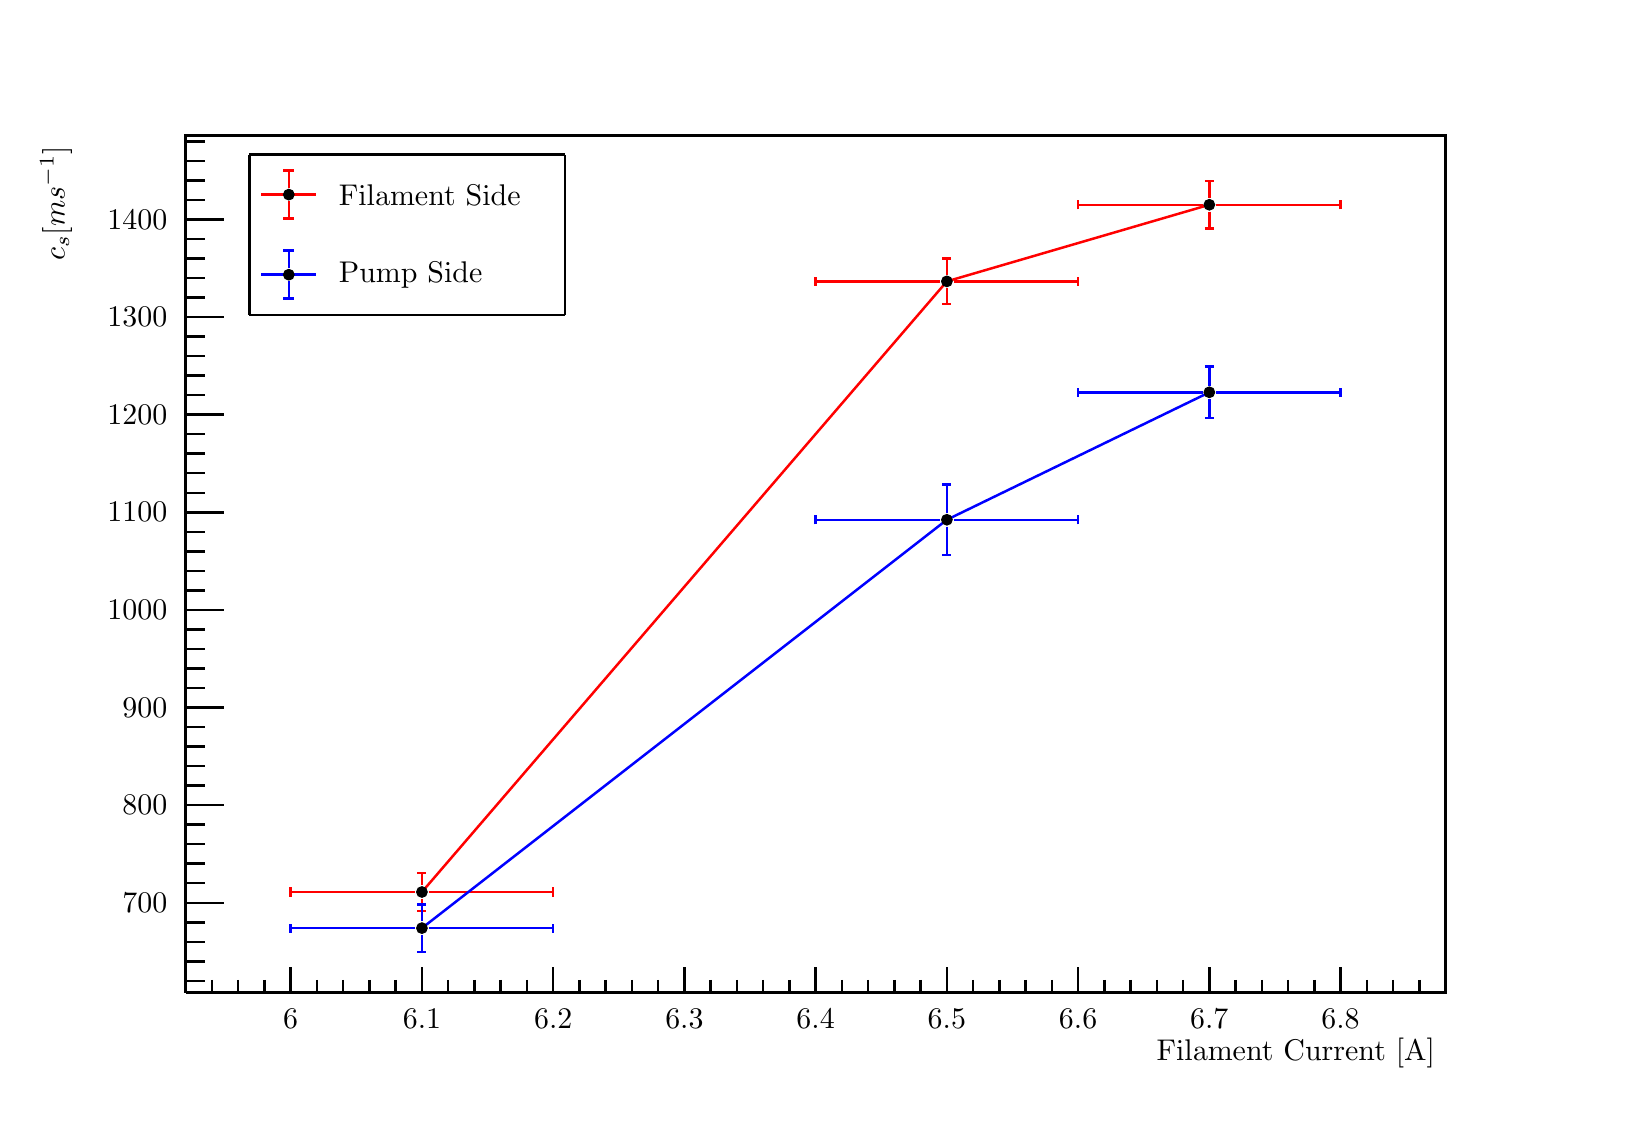
\begin{tikzpicture}
\pgfdeclareplotmark{cross} {
\pgfpathmoveto{\pgfpoint{-0.3\pgfplotmarksize}{\pgfplotmarksize}}
\pgfpathlineto{\pgfpoint{+0.3\pgfplotmarksize}{\pgfplotmarksize}}
\pgfpathlineto{\pgfpoint{+0.3\pgfplotmarksize}{0.3\pgfplotmarksize}}
\pgfpathlineto{\pgfpoint{+1\pgfplotmarksize}{0.3\pgfplotmarksize}}
\pgfpathlineto{\pgfpoint{+1\pgfplotmarksize}{-0.3\pgfplotmarksize}}
\pgfpathlineto{\pgfpoint{+0.3\pgfplotmarksize}{-0.3\pgfplotmarksize}}
\pgfpathlineto{\pgfpoint{+0.3\pgfplotmarksize}{-1.\pgfplotmarksize}}
\pgfpathlineto{\pgfpoint{-0.3\pgfplotmarksize}{-1.\pgfplotmarksize}}
\pgfpathlineto{\pgfpoint{-0.3\pgfplotmarksize}{-0.3\pgfplotmarksize}}
\pgfpathlineto{\pgfpoint{-1.\pgfplotmarksize}{-0.3\pgfplotmarksize}}
\pgfpathlineto{\pgfpoint{-1.\pgfplotmarksize}{0.3\pgfplotmarksize}}
\pgfpathlineto{\pgfpoint{-0.3\pgfplotmarksize}{0.3\pgfplotmarksize}}
\pgfpathclose
\pgfusepathqstroke
}
\pgfdeclareplotmark{cross*} {
\pgfpathmoveto{\pgfpoint{-0.3\pgfplotmarksize}{\pgfplotmarksize}}
\pgfpathlineto{\pgfpoint{+0.3\pgfplotmarksize}{\pgfplotmarksize}}
\pgfpathlineto{\pgfpoint{+0.3\pgfplotmarksize}{0.3\pgfplotmarksize}}
\pgfpathlineto{\pgfpoint{+1\pgfplotmarksize}{0.3\pgfplotmarksize}}
\pgfpathlineto{\pgfpoint{+1\pgfplotmarksize}{-0.3\pgfplotmarksize}}
\pgfpathlineto{\pgfpoint{+0.3\pgfplotmarksize}{-0.3\pgfplotmarksize}}
\pgfpathlineto{\pgfpoint{+0.3\pgfplotmarksize}{-1.\pgfplotmarksize}}
\pgfpathlineto{\pgfpoint{-0.3\pgfplotmarksize}{-1.\pgfplotmarksize}}
\pgfpathlineto{\pgfpoint{-0.3\pgfplotmarksize}{-0.3\pgfplotmarksize}}
\pgfpathlineto{\pgfpoint{-1.\pgfplotmarksize}{-0.3\pgfplotmarksize}}
\pgfpathlineto{\pgfpoint{-1.\pgfplotmarksize}{0.3\pgfplotmarksize}}
\pgfpathlineto{\pgfpoint{-0.3\pgfplotmarksize}{0.3\pgfplotmarksize}}
\pgfpathclose
\pgfusepathqfillstroke
}
\pgfdeclareplotmark{newstar} {
\pgfpathmoveto{\pgfqpoint{0pt}{\pgfplotmarksize}}
\pgfpathlineto{\pgfqpointpolar{44}{0.5\pgfplotmarksize}}
\pgfpathlineto{\pgfqpointpolar{18}{\pgfplotmarksize}}
\pgfpathlineto{\pgfqpointpolar{-20}{0.5\pgfplotmarksize}}
\pgfpathlineto{\pgfqpointpolar{-54}{\pgfplotmarksize}}
\pgfpathlineto{\pgfqpointpolar{-90}{0.5\pgfplotmarksize}}
\pgfpathlineto{\pgfqpointpolar{234}{\pgfplotmarksize}}
\pgfpathlineto{\pgfqpointpolar{198}{0.5\pgfplotmarksize}}
\pgfpathlineto{\pgfqpointpolar{162}{\pgfplotmarksize}}
\pgfpathlineto{\pgfqpointpolar{134}{0.5\pgfplotmarksize}}
\pgfpathclose
\pgfusepathqstroke
}
\pgfdeclareplotmark{newstar*} {
\pgfpathmoveto{\pgfqpoint{0pt}{\pgfplotmarksize}}
\pgfpathlineto{\pgfqpointpolar{44}{0.5\pgfplotmarksize}}
\pgfpathlineto{\pgfqpointpolar{18}{\pgfplotmarksize}}
\pgfpathlineto{\pgfqpointpolar{-20}{0.5\pgfplotmarksize}}
\pgfpathlineto{\pgfqpointpolar{-54}{\pgfplotmarksize}}
\pgfpathlineto{\pgfqpointpolar{-90}{0.5\pgfplotmarksize}}
\pgfpathlineto{\pgfqpointpolar{234}{\pgfplotmarksize}}
\pgfpathlineto{\pgfqpointpolar{198}{0.5\pgfplotmarksize}}
\pgfpathlineto{\pgfqpointpolar{162}{\pgfplotmarksize}}
\pgfpathlineto{\pgfqpointpolar{134}{0.5\pgfplotmarksize}}
\pgfpathclose
\pgfusepathqfillstroke
}
\definecolor{c}{rgb}{1,1,1};
\draw [color=c, fill=c] (0,0) rectangle (20,13.6103);
\draw [color=c, fill=c] (2,1.36103) rectangle (18,12.2493);
\definecolor{c}{rgb}{0,0,0};
\draw [c,line width=0.9] (2,1.36103) -- (2,12.2493) -- (18,12.2493) -- (18,1.36103) -- (2,1.36103);
\definecolor{c}{rgb}{1,1,1};
\draw [color=c, fill=c] (2,1.36103) rectangle (18,12.2493);
\definecolor{c}{rgb}{0,0,0};
\draw [c,line width=0.9] (2,1.36103) -- (2,12.2493) -- (18,12.2493) -- (18,1.36103) -- (2,1.36103);
\draw [c,line width=0.9] (2,1.36103) -- (18,1.36103);
\draw [c,line width=0.9] (3.33333,1.68768) -- (3.33333,1.36103);
\draw [c,line width=0.9] (3.66667,1.52436) -- (3.66667,1.36103);
\draw [c,line width=0.9] (4,1.52436) -- (4,1.36103);
\draw [c,line width=0.9] (4.33333,1.52436) -- (4.33333,1.36103);
\draw [c,line width=0.9] (4.66667,1.52436) -- (4.66667,1.36103);
\draw [c,line width=0.9] (5,1.68768) -- (5,1.36103);
\draw [c,line width=0.9] (5.33333,1.52436) -- (5.33333,1.36103);
\draw [c,line width=0.9] (5.66667,1.52436) -- (5.66667,1.36103);
\draw [c,line width=0.9] (6,1.52436) -- (6,1.36103);
\draw [c,line width=0.9] (6.33333,1.52436) -- (6.33333,1.36103);
\draw [c,line width=0.9] (6.66667,1.68768) -- (6.66667,1.36103);
\draw [c,line width=0.9] (7,1.52436) -- (7,1.36103);
\draw [c,line width=0.9] (7.33333,1.52436) -- (7.33333,1.36103);
\draw [c,line width=0.9] (7.66667,1.52436) -- (7.66667,1.36103);
\draw [c,line width=0.9] (8,1.52436) -- (8,1.36103);
\draw [c,line width=0.9] (8.33333,1.68768) -- (8.33333,1.36103);
\draw [c,line width=0.9] (8.66667,1.52436) -- (8.66667,1.36103);
\draw [c,line width=0.9] (9,1.52436) -- (9,1.36103);
\draw [c,line width=0.9] (9.33333,1.52436) -- (9.33333,1.36103);
\draw [c,line width=0.9] (9.66667,1.52436) -- (9.66667,1.36103);
\draw [c,line width=0.9] (10,1.68768) -- (10,1.36103);
\draw [c,line width=0.9] (10.3333,1.52436) -- (10.3333,1.36103);
\draw [c,line width=0.9] (10.6667,1.52436) -- (10.6667,1.36103);
\draw [c,line width=0.9] (11,1.52436) -- (11,1.36103);
\draw [c,line width=0.9] (11.3333,1.52436) -- (11.3333,1.36103);
\draw [c,line width=0.9] (11.6667,1.68768) -- (11.6667,1.36103);
\draw [c,line width=0.9] (12,1.52436) -- (12,1.36103);
\draw [c,line width=0.9] (12.3333,1.52436) -- (12.3333,1.36103);
\draw [c,line width=0.9] (12.6667,1.52436) -- (12.6667,1.36103);
\draw [c,line width=0.9] (13,1.52436) -- (13,1.36103);
\draw [c,line width=0.9] (13.3333,1.68768) -- (13.3333,1.36103);
\draw [c,line width=0.9] (13.6667,1.52436) -- (13.6667,1.36103);
\draw [c,line width=0.9] (14,1.52436) -- (14,1.36103);
\draw [c,line width=0.9] (14.3333,1.52436) -- (14.3333,1.36103);
\draw [c,line width=0.9] (14.6667,1.52436) -- (14.6667,1.36103);
\draw [c,line width=0.9] (15,1.68768) -- (15,1.36103);
\draw [c,line width=0.9] (15.3333,1.52436) -- (15.3333,1.36103);
\draw [c,line width=0.9] (15.6667,1.52436) -- (15.6667,1.36103);
\draw [c,line width=0.9] (16,1.52436) -- (16,1.36103);
\draw [c,line width=0.9] (16.3333,1.52436) -- (16.3333,1.36103);
\draw [c,line width=0.9] (16.6667,1.68768) -- (16.6667,1.36103);
\draw [c,line width=0.9] (3.33333,1.68768) -- (3.33333,1.36103);
\draw [c,line width=0.9] (3,1.52436) -- (3,1.36103);
\draw [c,line width=0.9] (2.66667,1.52436) -- (2.66667,1.36103);
\draw [c,line width=0.9] (2.33333,1.52436) -- (2.33333,1.36103);
\draw [c,line width=0.9] (2,1.52436) -- (2,1.36103);
\draw [c,line width=0.9] (16.6667,1.68768) -- (16.6667,1.36103);
\draw [c,line width=0.9] (17,1.52436) -- (17,1.36103);
\draw [c,line width=0.9] (17.3333,1.52436) -- (17.3333,1.36103);
\draw [c,line width=0.9] (17.6667,1.52436) -- (17.6667,1.36103);
\draw [anchor=base] (3.33333,0.911891) node[scale=1.08185, color=c, rotate=0]{6};
\draw [anchor=base] (5,0.911891) node[scale=1.08185, color=c, rotate=0]{6.1};
\draw [anchor=base] (6.66667,0.911891) node[scale=1.08185, color=c, rotate=0]{6.2};
\draw [anchor=base] (8.33333,0.911891) node[scale=1.08185, color=c, rotate=0]{6.3};
\draw [anchor=base] (10,0.911891) node[scale=1.08185, color=c, rotate=0]{6.4};
\draw [anchor=base] (11.6667,0.911891) node[scale=1.08185, color=c, rotate=0]{6.5};
\draw [anchor=base] (13.3333,0.911891) node[scale=1.08185, color=c, rotate=0]{6.6};
\draw [anchor=base] (15,0.911891) node[scale=1.08185, color=c, rotate=0]{6.7};
\draw [anchor=base] (16.6667,0.911891) node[scale=1.08185, color=c, rotate=0]{6.8};
\draw [anchor= east] (18,0.598854) node[scale=1.08185, color=c, rotate=0]{Filament Current [A]};
\draw [c,line width=0.9] (2,1.36103) -- (2,12.2493);
\draw [c,line width=0.9] (2.48,2.5036) -- (2,2.5036);
\draw [c,line width=0.9] (2.24,2.75156) -- (2,2.75156);
\draw [c,line width=0.9] (2.24,2.99952) -- (2,2.99952);
\draw [c,line width=0.9] (2.24,3.24748) -- (2,3.24748);
\draw [c,line width=0.9] (2.24,3.49544) -- (2,3.49544);
\draw [c,line width=0.9] (2.48,3.7434) -- (2,3.7434);
\draw [c,line width=0.9] (2.24,3.99137) -- (2,3.99137);
\draw [c,line width=0.9] (2.24,4.23933) -- (2,4.23933);
\draw [c,line width=0.9] (2.24,4.48729) -- (2,4.48729);
\draw [c,line width=0.9] (2.24,4.73525) -- (2,4.73525);
\draw [c,line width=0.9] (2.48,4.98321) -- (2,4.98321);
\draw [c,line width=0.9] (2.24,5.23117) -- (2,5.23117);
\draw [c,line width=0.9] (2.24,5.47913) -- (2,5.47913);
\draw [c,line width=0.9] (2.24,5.72709) -- (2,5.72709);
\draw [c,line width=0.9] (2.24,5.97505) -- (2,5.97505);
\draw [c,line width=0.9] (2.48,6.22301) -- (2,6.22301);
\draw [c,line width=0.9] (2.24,6.47097) -- (2,6.47097);
\draw [c,line width=0.9] (2.24,6.71893) -- (2,6.71893);
\draw [c,line width=0.9] (2.24,6.96689) -- (2,6.96689);
\draw [c,line width=0.9] (2.24,7.21485) -- (2,7.21485);
\draw [c,line width=0.9] (2.48,7.46281) -- (2,7.46281);
\draw [c,line width=0.9] (2.24,7.71077) -- (2,7.71077);
\draw [c,line width=0.9] (2.24,7.95873) -- (2,7.95873);
\draw [c,line width=0.9] (2.24,8.20669) -- (2,8.20669);
\draw [c,line width=0.9] (2.24,8.45465) -- (2,8.45465);
\draw [c,line width=0.9] (2.48,8.70261) -- (2,8.70261);
\draw [c,line width=0.9] (2.24,8.95057) -- (2,8.95057);
\draw [c,line width=0.9] (2.24,9.19854) -- (2,9.19854);
\draw [c,line width=0.9] (2.24,9.4465) -- (2,9.4465);
\draw [c,line width=0.9] (2.24,9.69446) -- (2,9.69446);
\draw [c,line width=0.9] (2.48,9.94242) -- (2,9.94242);
\draw [c,line width=0.9] (2.24,10.1904) -- (2,10.1904);
\draw [c,line width=0.9] (2.24,10.4383) -- (2,10.4383);
\draw [c,line width=0.9] (2.24,10.6863) -- (2,10.6863);
\draw [c,line width=0.9] (2.24,10.9343) -- (2,10.9343);
\draw [c,line width=0.9] (2.48,11.1822) -- (2,11.1822);
\draw [c,line width=0.9] (2.48,2.5036) -- (2,2.5036);
\draw [c,line width=0.9] (2.24,2.25564) -- (2,2.25564);
\draw [c,line width=0.9] (2.24,2.00768) -- (2,2.00768);
\draw [c,line width=0.9] (2.24,1.75972) -- (2,1.75972);
\draw [c,line width=0.9] (2.24,1.51176) -- (2,1.51176);
\draw [c,line width=0.9] (2.48,11.1822) -- (2,11.1822);
\draw [c,line width=0.9] (2.24,11.4302) -- (2,11.4302);
\draw [c,line width=0.9] (2.24,11.6781) -- (2,11.6781);
\draw [c,line width=0.9] (2.24,11.9261) -- (2,11.9261);
\draw [c,line width=0.9] (2.24,12.1741) -- (2,12.1741);
\draw [anchor= east] (1.9,2.5036) node[scale=1.08185, color=c, rotate=0]{700};
\draw [anchor= east] (1.9,3.7434) node[scale=1.08185, color=c, rotate=0]{800};
\draw [anchor= east] (1.9,4.98321) node[scale=1.08185, color=c, rotate=0]{900};
\draw [anchor= east] (1.9,6.22301) node[scale=1.08185, color=c, rotate=0]{1000};
\draw [anchor= east] (1.9,7.46281) node[scale=1.08185, color=c, rotate=0]{1100};
\draw [anchor= east] (1.9,8.70261) node[scale=1.08185, color=c, rotate=0]{1200};
\draw [anchor= east] (1.9,9.94242) node[scale=1.08185, color=c, rotate=0]{1300};
\draw [anchor= east] (1.9,11.1822) node[scale=1.08185, color=c, rotate=0]{1400};
\draw [anchor= east] (0.354441,12.2493) node[scale=1.08185, color=c, rotate=90]{$c_s [m s^{-1}]$};
\definecolor{c}{rgb}{1,0,0};
\draw [c,line width=0.9] (5,2.64038) -- (11.6667,10.3952) -- (15,11.3682);
\definecolor{c}{rgb}{0,0,0};
\foreach \P in {(5,2.64038), (11.6667,10.3952), (15,11.3682)}{\draw[mark options={color=c,fill=c},mark size=1.921922pt,mark=*] plot coordinates {\P};}
\definecolor{c}{rgb}{1,0,0};
\draw [c,line width=0.9] (4.91404,2.64038) -- (3.33333,2.64038);
\draw [c,line width=0.9] (3.33333,2.58307) -- (3.33333,2.69768);
\draw [c,line width=0.9] (5.08596,2.64038) -- (6.66667,2.64038);
\draw [c,line width=0.9] (6.66667,2.58307) -- (6.66667,2.69768);
\draw [c,line width=0.9] (5,2.72634) -- (5,2.88022);
\draw [c,line width=0.9] (4.94269,2.88022) -- (5.05731,2.88022);
\draw [c,line width=0.9] (5,2.55442) -- (5,2.40053);
\draw [c,line width=0.9] (4.94269,2.40053) -- (5.05731,2.40053);
\draw [c,line width=0.9] (11.5807,10.3952) -- (10,10.3952);
\draw [c,line width=0.9] (10,10.3379) -- (10,10.4525);
\draw [c,line width=0.9] (11.7526,10.3952) -- (13.3333,10.3952);
\draw [c,line width=0.9] (13.3333,10.3379) -- (13.3333,10.4525);
\draw [c,line width=0.9] (11.6667,10.4812) -- (11.6667,10.6834);
\draw [c,line width=0.9] (11.6094,10.6834) -- (11.724,10.6834);
\draw [c,line width=0.9] (11.6667,10.3092) -- (11.6667,10.107);
\draw [c,line width=0.9] (11.6094,10.107) -- (11.724,10.107);
\draw [c,line width=0.9] (14.914,11.3682) -- (13.3333,11.3682);
\draw [c,line width=0.9] (13.3333,11.3109) -- (13.3333,11.4255);
\draw [c,line width=0.9] (15.086,11.3682) -- (16.6667,11.3682);
\draw [c,line width=0.9] (16.6667,11.3109) -- (16.6667,11.4255);
\draw [c,line width=0.9] (15,11.4541) -- (15,11.6701);
\draw [c,line width=0.9] (14.9427,11.6701) -- (15.0573,11.6701);
\draw [c,line width=0.9] (15,11.2822) -- (15,11.0663);
\draw [c,line width=0.9] (14.9427,11.0663) -- (15.0573,11.0663);
\definecolor{c}{rgb}{0,0,1};
\draw [c,line width=0.9] (4.91404,2.18174) -- (3.33333,2.18174);
\draw [c,line width=0.9] (3.33333,2.12443) -- (3.33333,2.23904);
\draw [c,line width=0.9] (5.08596,2.18174) -- (6.66667,2.18174);
\draw [c,line width=0.9] (6.66667,2.12443) -- (6.66667,2.23904);
\draw [c,line width=0.9] (5,2.2677) -- (5,2.48277);
\draw [c,line width=0.9] (4.94269,2.48277) -- (5.05731,2.48277);
\draw [c,line width=0.9] (5,2.09578) -- (5,1.88071);
\draw [c,line width=0.9] (4.94269,1.88071) -- (5.05731,1.88071);
\draw [c,line width=0.9] (11.5807,7.36784) -- (10,7.36784);
\draw [c,line width=0.9] (10,7.31054) -- (10,7.42515);
\draw [c,line width=0.9] (11.7526,7.36784) -- (13.3333,7.36784);
\draw [c,line width=0.9] (13.3333,7.31054) -- (13.3333,7.42515);
\draw [c,line width=0.9] (11.6667,7.4538) -- (11.6667,7.81722);
\draw [c,line width=0.9] (11.6094,7.81722) -- (11.724,7.81722);
\draw [c,line width=0.9] (11.6667,7.28188) -- (11.6667,6.91847);
\draw [c,line width=0.9] (11.6094,6.91847) -- (11.724,6.91847);
\draw [c,line width=0.9] (14.914,8.98653) -- (13.3333,8.98653);
\draw [c,line width=0.9] (13.3333,8.92922) -- (13.3333,9.04384);
\draw [c,line width=0.9] (15.086,8.98653) -- (16.6667,8.98653);
\draw [c,line width=0.9] (16.6667,8.92922) -- (16.6667,9.04384);
\draw [c,line width=0.9] (15,9.07249) -- (15,9.31458);
\draw [c,line width=0.9] (14.9427,9.31458) -- (15.0573,9.31458);
\draw [c,line width=0.9] (15,8.90057) -- (15,8.65848);
\draw [c,line width=0.9] (14.9427,8.65848) -- (15.0573,8.65848);
\draw [c,line width=0.9] (5,2.18174) -- (11.6667,7.36784) -- (15,8.98653);
\definecolor{c}{rgb}{0,0,0};
\foreach \P in {(5,2.18174), (11.6667,7.36784), (15,8.98653)}{\draw[mark options={color=c,fill=c},mark size=1.921922pt,mark=*] plot coordinates {\P};}
\definecolor{c}{rgb}{1,1,1};
\draw [color=c, fill=c] (2.80802,9.97135) rectangle (6.81948,12.0057);
\definecolor{c}{rgb}{0,0,0};
\draw [c,line width=0.9] (2.80802,9.97135) -- (6.81948,9.97135);
\draw [c,line width=0.9] (6.81948,9.97135) -- (6.81948,12.0057);
\draw [c,line width=0.9] (6.81948,12.0057) -- (2.80802,12.0057);
\draw [c,line width=0.9] (2.80802,12.0057) -- (2.80802,9.97135);
\draw [anchor= west] (3.81089,11.4971) node[scale=1.08185, color=c, rotate=0]{Filament Side};
\definecolor{c}{rgb}{1,0,0};
\draw [c,line width=0.9] (2.95845,11.4971) -- (3.66046,11.4971);
\draw [c,line width=0.9] (3.30946,11.5831) -- (3.30946,11.8023);
\draw [c,line width=0.9] (3.30946,11.4112) -- (3.30946,11.192);
\draw [c,line width=0.9] (3.23925,11.8023) -- (3.37966,11.8023);
\draw [c,line width=0.9] (3.23925,11.192) -- (3.37966,11.192);
\definecolor{c}{rgb}{0,0,0};
\foreach \P in {(3.30946,11.4971)}{\draw[mark options={color=c,fill=c},mark size=1.921922pt,mark=*] plot coordinates {\P};}
\draw [anchor= west] (3.81089,10.4799) node[scale=1.08185, color=c, rotate=0]{Pump Side};
\definecolor{c}{rgb}{0,0,1};
\draw [c,line width=0.9] (2.95845,10.4799) -- (3.66046,10.4799);
\draw [c,line width=0.9] (3.30946,10.5659) -- (3.30946,10.7851);
\draw [c,line width=0.9] (3.30946,10.394) -- (3.30946,10.1748);
\draw [c,line width=0.9] (3.23925,10.7851) -- (3.37966,10.7851);
\draw [c,line width=0.9] (3.23925,10.1748) -- (3.37966,10.1748);
\definecolor{c}{rgb}{0,0,0};
\foreach \P in {(3.30946,10.4799)}{\draw[mark options={color=c,fill=c},mark size=1.921922pt,mark=*] plot coordinates {\P};}
\end{tikzpicture}
